%%
%% This is file `sample-sigplan.tex',
%% generated with the docstrip utility.
%%
%% The original source files were:
%%
%% samples.dtx  (with options: `sigplan')
%% 
%% IMPORTANT NOTICE:
%% 
%% For the copyright see the source file.
%% 
%% Any modified versions of this file must be renamed
%% with new filenames distinct from sample-sigplan.tex.
%% 
%% For distribution of the original source see the terms
%% for copying and modification in the file samples.dtx.
%% 
%% This generated file may be distributed as long as the
%% original source files, as listed above, are part of the
%% same distribution. (The sources need not necessarily be
%% in the same archive or directory.)
%%
%% The first command in your LaTeX source must be the \documentclass command.
\documentclass[sigplan,screen,nonacm]{acmart}
\usepackage{color}
\usepackage[colorinlistoftodos]{todonotes}
\usepackage[
    type={CC},
    modifier={by-nc-sa},
    version={4.0},
]{doclicense}
%% NOTE that a single column version is required for 
%% submission and peer review. This can be done by changing
%% the \doucmentclass[...]{acmart} in this template to 
%% \documentclass[manuscript,screen,review]{acmart}
%% 
%% To ensure 100% compatibility, please check the white list of
%% approved LaTeX packages to be used with the Master Article Template at
%% https://www.acm.org/publications/taps/whitelist-of-latex-packages 
%% before creating your document. The white list page provides 
%% information on how to submit additional LaTeX packages for 
%% review and adoption.
%% Fonts used in the template cannot be substituted; margin 
%% adjustments are not allowed.
%%
%% \BibTeX command to typeset BibTeX logo in the docs
\AtBeginDocument{%
  \providecommand\BibTeX{{%
    \normalfont B\kern-0.5em{\scshape i\kern-0.25em b}\kern-0.8em\TeX}}}


%%
%% end of the preamble, start of the body of the document source.
\begin{document}

%%
%% The "title" command has an optional parameter,
%% allowing the author to define a "short title" to be used in page headers.
\title{Sample Paper}

%%
%% The "author" command and its associated commands are used to define
%% the authors and their affiliations.
%% Of note is the shared affiliation of the first two authors, and the
%% "authornote" and "authornotemark" commands
%% used to denote shared contribution to the research.
\author{Cole N. Maxwell}
\email{maxwe206@morris.umn.edu}
\affiliation{%
  \institution{Division of Science and Mathematics 
	\\
        University of Minnesota, Morris
	}
  \city{Morris}
  \state{Minnesota}
  \country{USA}
  \postcode{56267}
}

%%
%% By default, the full list of authors will be used in the page
%% headers. Often, this list is too long, and will overlap
%% other information printed in the page headers. This command allows
%% the author to define a more concise list
%% of authors' names for this purpose.
%\renewcommand{\shortauthors}{Trovato and Tobin, et al.}

%%
%% The abstract is a short summary of the work to be presented in the
%% article.
\begin{abstract}
This paper provides a sample of a \LaTeX\ document which conforms,
somewhat loosely, to the formatting guidelines for the University of
Minnesota, Morris, Computer Science Senior Seminar proceedings.
It is based heavily on (and takes material directly from) a similar document 
illustrating the format of the ACM SIG Proceedings, which we have based our
proceedings format on.

The original ACM document tried to include
\begin{quote}
every imaginable sort
of ``bells and whistles", such as a subtitle, footnotes on
title, subtitle and authors, as well as in the text, and
every optional component (e.g. Acknowledgments, Additional
Authors, Appendices), not to mention examples of
equations, theorems, tables and figures.
\end{quote}

We've removed many of the more esoteric tricks here because either
they'll never be used (e.g., multiple authors) or are used \emph{very}
rarely (e.g., appendices). Refer to the original ACM document for more
of those fancy examples.
\todo[inline]{You can add comments, such as: Needs more work}
\end{abstract}

\doclicenseThis

%%
%% Keywords. The author(s) should pick words that accurately describe
%% the work being presented. Separate the keywords with commas.
\keywords{datasets, neural networks, gaze detection, text tagging}


%%
%% This command processes the author and affiliation and title
%% information and builds the first part of the formatted document.
\maketitle

\section{Introduction}
\label{sec:introduction}

The \textit{proceedings} are the records of a conference, and conference
editors like ACM seek to give their conference by-products a uniform,
high-quality appearance. We also would like our proceedings to look highly
professional, so we're borrowing heavily from the ACM formatting guidelines.
These include some
rigid requirements for the format of the proceedings documents: there
is a specified format (balanced  double columns), a specified
set of fonts (Arial or Helvetica and Times Roman) in
certain specified sizes (for instance, 9 point for body copy),
a specified live area (18 $\times$ 23.5 cm [7" $\times$ 9.25"]) centered on
the page, specified size of margins (2.54cm [1"] top and
bottom and 1.9cm [.75"] left and right; specified column width
(8.45cm [3.33"]) and gutter size (.083cm [.33"]).

\todo[inline, color=green]{I really like this section.}

The good news is, with only a handful of manual
settings the \LaTeX\ document
class file\footnote{Look at the \texttt{documentclass} in the beginning to see what it is.} handles all of this for you.

The remainder of this document is concerned with showing, in
the context of an ``actual'' document, the \LaTeX\ commands
specifically available for denoting the structure of a
proceedings paper, rather than with giving rigorous descriptions
or explanations of such commands. Section~\ref{sec:body} introduces the main
examples of formatting, and Section~\ref{sec:conclusions} wraps things up. 

\section{The {\it Body} of The Paper}
\label{sec:body}

Typically, the body of a paper is organized
into a hierarchical structure, with numbered or unnumbered
headings for sections, subsections, sub-subsections, and even
smaller sections.  The command \texttt{\textbackslash section} that
precedes this paragraph is part of such a
hierarchy.\footnote{This is the second footnote.  It
starts a series of three footnotes that add nothing
informational, but just give an idea of how footnotes work
and look. It is a wordy one, just so you see
how a longish one plays out.} \LaTeX\ handles the numbering
and placement of these headings for you, when you use
the appropriate heading commands around the titles
of the headings.  If you want a sub-subsection or
smaller part to be unnumbered in your output, simply append an
asterisk to the command name.  Examples of both
numbered and unnumbered headings will appear throughout the
balance of this sample document.

Because the entire article is contained in
the \textbf{document} environment, you can indicate the
start of a new paragraph with a blank line in your
input file; that is why this sentence forms a separate paragraph.

\subsection{Type Changes and {\it Special} Characters}
\label{sec:typeChangesSpecialChars}

We have already seen several typeface changes in this sample.  You
can indicate italicized words or phrases in your text with
the command \texttt{\textbackslash textit}; emboldening with the
command \texttt{\textbackslash textbf}
and typewriter-style (for instance, for computer code) with
\texttt{\textbackslash texttt}.
As a rule you'd prefer \texttt{\textbackslash emph} (which stands for \emph{emphasize})
over something like \texttt{\textbackslash textit} since that gives the typesetting system
more flexibility in how it can emphasize that text.

You do not
have to indicate typestyle changes when such changes are
part of the \textit{structural} elements of your
article; for instance, the heading of this subsection will
be in a sans serif\footnote{A third footnote, here.
Let's make this a rather short one to
see how it looks.} typeface, but that is handled by the
document class file. Take care with the use
of\footnote{A fourth, and last, footnote.}
the curly braces in typeface changes; they mark
the beginning and end of
the text that is to be in the different typeface.

You can use whatever symbols, accented characters, or
non-English characters you need anywhere in your document;
you can find a complete list of what is
available in the \textit{\LaTeX\
User's Guide}~\cite{Lamport:LaTeX}.


\section{Sectioning Commands}

Your work should use standard \LaTeX\ sectioning commands:
\verb|section|, \verb|subsection|, \verb|subsubsection|, and
\verb|paragraph|. They should be numbered; do not remove the numbering
from the commands.

Simulating a sectioning command by setting the first word or words of
a paragraph in boldface or italicized text is {\bfseries not allowed.}

\section{Tables}

The ``\verb|acmart|'' document class includes the ``\verb|booktabs|''
package --- \url{https://ctan.org/pkg/booktabs} --- for preparing
high-quality tables.

Table captions are placed {\itshape above} the table.

Because tables cannot be split across pages, the best placement for
them is typically the top of the page nearest their initial cite.  To
ensure this proper ``floating'' placement of tables, use the
environment \textbf{table} to enclose the table's contents and the
table caption.  The contents of the table itself must go in the
\textbf{tabular} environment, to be aligned properly in rows and
columns, with the desired horizontal and vertical rules.  Again,
detailed instructions on \textbf{tabular} material are found in the
\textit{\LaTeX\ User's Guide}.

Immediately following this sentence is the point at which
Table~\ref{tab:freq} is included in the input file; compare the
placement of the table here with the table in the printed output of
this document.

\begin{table}
  \caption{Frequency of Special Characters}
  \label{tab:freq}
  \begin{tabular}{ccl}
    \toprule
    Non-English or Math&Frequency&Comments\\
    \midrule
    \O & 1 in 1,000& For Swedish names\\
    $\pi$ & 1 in 5& Common in math\\
    \$ & 4 in 5 & Used in business\\
    $\Psi^2_1$ & 1 in 40,000& Unexplained usage\\
  \bottomrule
\end{tabular}
\end{table}

To set a wider table, which takes up the whole width of the page's
live area, use the environment \textbf{table*} to enclose the table's
contents and the table caption.  As with a single-column table, this
wide table will ``float'' to a location deemed more
desirable. Immediately following this sentence is the point at which
Table~\ref{tab:commands} is included in the input file; again, it is
instructive to compare the placement of the table here with the table
in the printed output of this document.

\begin{table*}
  \caption{Some Typical Commands}
  \label{tab:commands}
  \begin{tabular}{ccl}
    \toprule
    Command &A Number & Comments\\
    \midrule
    \texttt{{\char'134}author} & 100& Author \\
    \texttt{{\char'134}table}& 300 & For tables\\
    \texttt{{\char'134}table*}& 400& For wider tables\\
    \bottomrule
  \end{tabular}
\end{table*}

Always use midrule to separate table header rows from data rows, and
use it only for this purpose. This enables assistive technologies to
recognise table headers and support their users in navigating tables
more easily.

\section{Math Equations}
You may want to display math equations in three distinct styles:
inline, numbered or non-numbered display.  Each of the three are
discussed in the next sections.

\subsection{Inline (In-text) Equations}
A formula that appears in the running text is called an inline or
in-text formula.  It is produced by the \textbf{math} environment,
which can be invoked with the usual
\texttt{{\char'134}begin\,\ldots{\char'134}end} construction or with
the short form \texttt{\$\,\ldots\$}. You can use any of the symbols
and structures, from $\alpha$ to $\omega$, available in
\LaTeX~\cite{Lamport:LaTeX}; this section will simply show a few
examples of in-text equations in context. Notice how this equation:
\begin{math}
  \lim_{n\rightarrow \infty}x=0
\end{math},
set here in in-line math style, looks slightly different when
set in display style.  (See next section).

\subsection{Display Equations}
A numbered display equation---one set off by vertical space from the
text and centered horizontally---is produced by the \textbf{equation}
environment. An unnumbered display equation is produced by the
\textbf{displaymath} environment.

Again, in either environment, you can use any of the symbols and
structures available in \LaTeX\@; this section will just give a couple
of examples of display equations in context.  First, consider the
equation, shown as an inline equation above:
\begin{equation}
  \lim_{n\rightarrow \infty}x=0
\end{equation}
Notice how it is formatted somewhat differently in
the \textbf{displaymath}
environment.  Now, we'll enter an unnumbered equation:
\begin{displaymath}
  \sum_{i=0}^{\infty} x + 1
\end{displaymath}
and follow it with another numbered equation:
\begin{equation}
  \sum_{i=0}^{\infty}x_i=\int_{0}^{\pi+2} f
\end{equation}
just to demonstrate \LaTeX's able handling of numbering.

%\section{Figures}

%% Elena: this will be helpful to show eventually

%The ``\verb|figure|'' environment should be used for figures. One or
%more images can be placed within a figure. 

%If your figure contains
%third-party material, you must clearly identify it as such, as shown
%in the example below.
%\begin{figure}[h]
%  \centering
%  \includegraphics[width=\linewidth]{sample-franklin}
%  \caption{1907 Franklin Model D roadster. Photograph by Harris \&
%    Ewing, Inc. [Public domain], via Wikimedia
%    Commons. (\url{https://goo.gl/VLCRBB}).}
%  \Description{A woman and a girl in white dresses sit in an open car.}
%\end{figure}

\subsection{Figures}
\label{sec:figures}

Like tables, figures cannot be split across pages; the
best placement for them
is typically the top or the bottom of the page nearest
their initial cite.  To ensure this proper ``floating'' placement
of figures, use the environment
\textbf{figure} to enclose the figure and its caption.

This sample document contains examples of
a \textbf{.pdf} file to be displayable with \LaTeX, such as
Figure~\ref{fig:singleColumnFigure}.  More
details on each of these is found in the \textit{Author's Guide}.

\begin{figure}
\centering
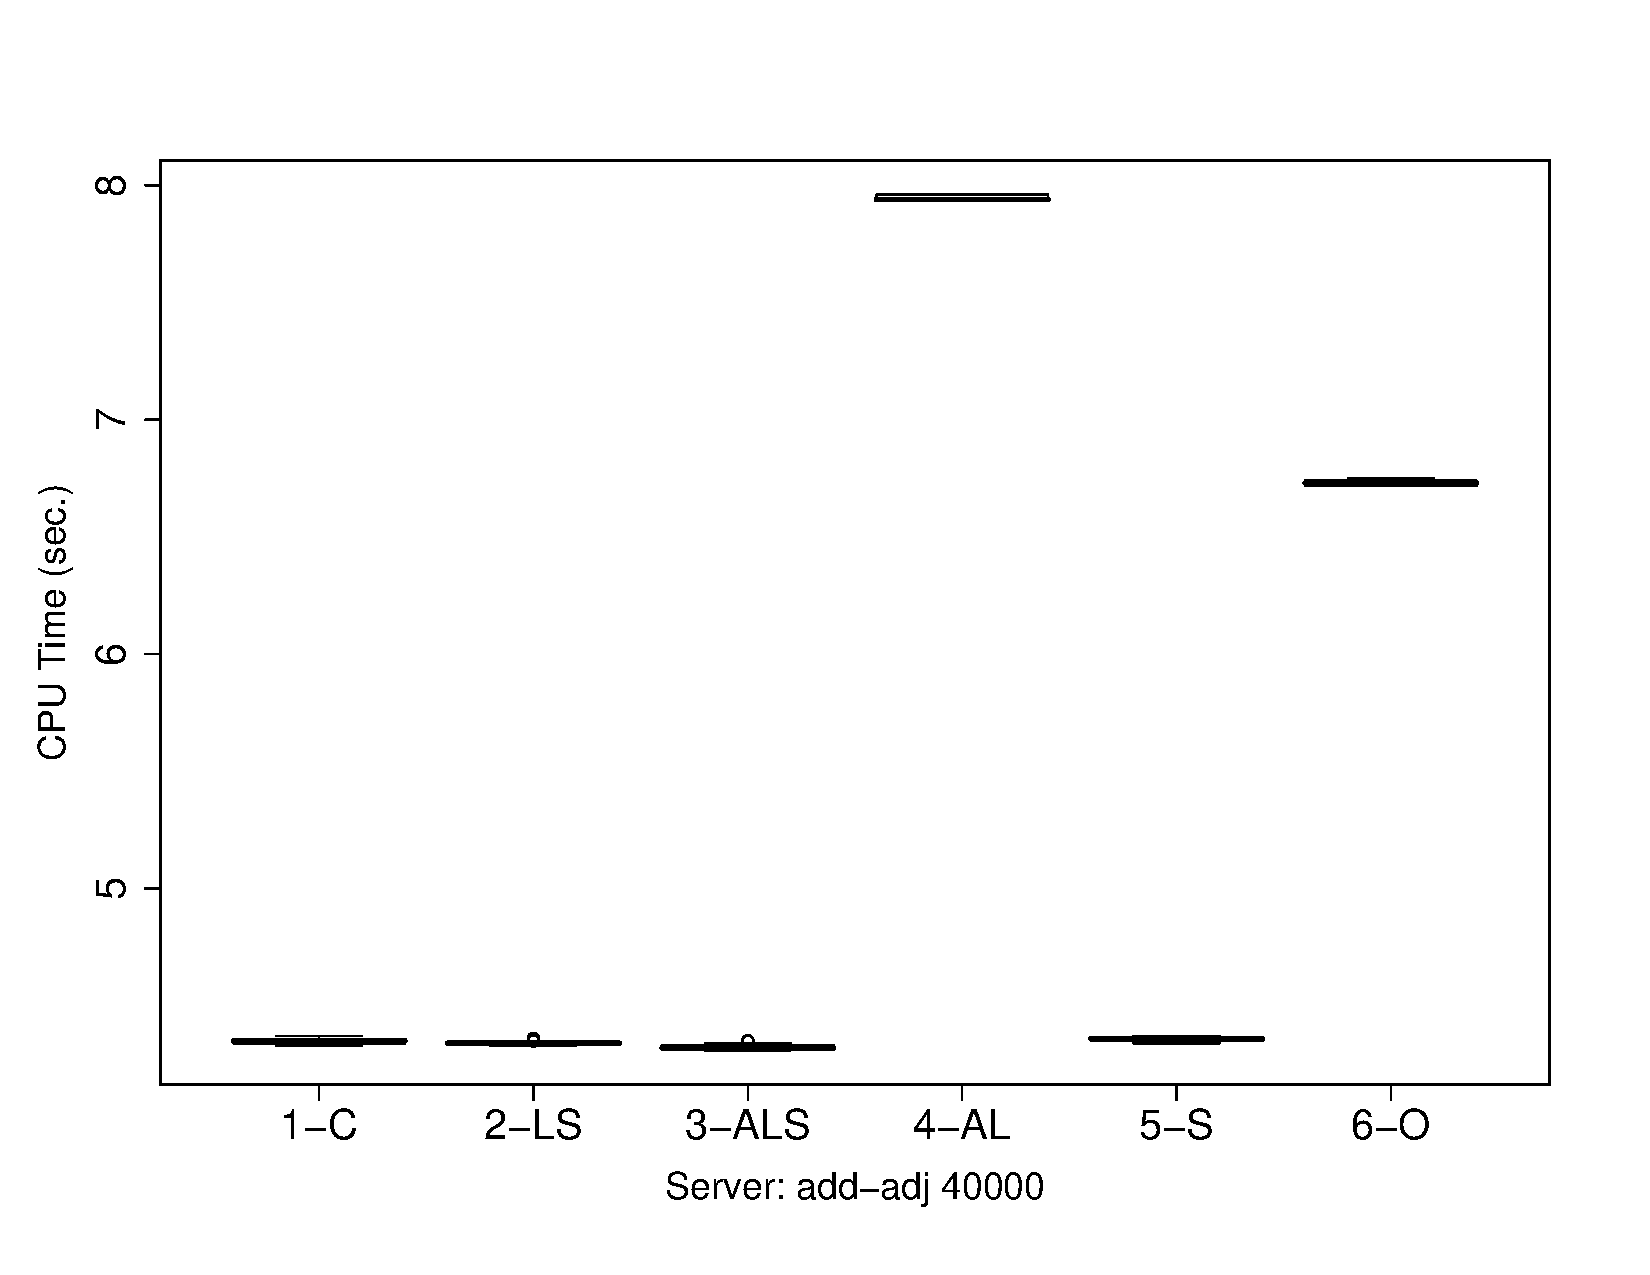
\includegraphics[width=3in]{sample_graph.pdf}
\caption{A sample graph just spanning one column.}
\Description{Describe your image for visually impaired}
\label{fig:singleColumnFigure}
\end{figure}


As was the case with tables, you may want a figure
that spans two columns, like Figure~\ref{fig:twoColumnFigure}.  
To do this, and still to
ensure proper ``floating'' placement of tables, use the environment
\texttt{figure*} to enclose the figure and its caption.
And don't forget to end the environment with
\texttt{figure*}, not \texttt{figure}!

\begin{figure*}
\centering
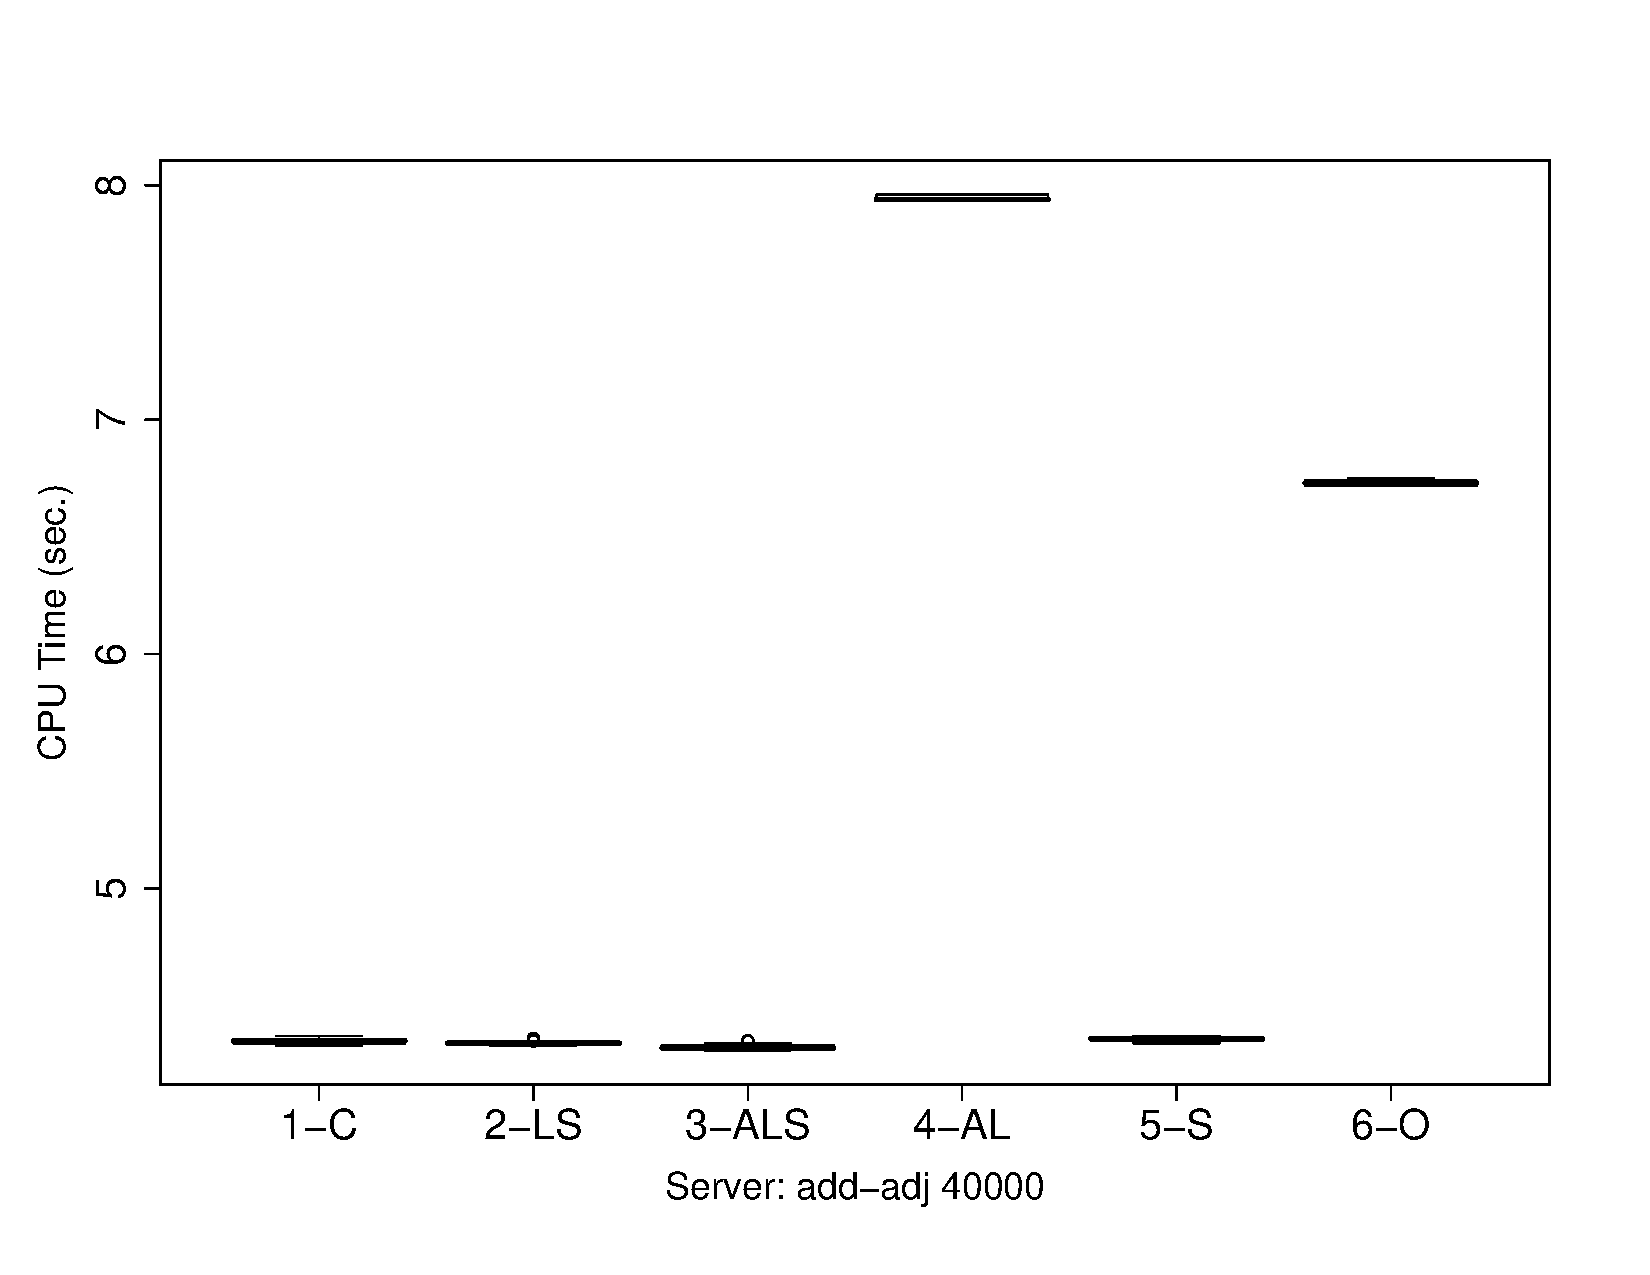
\includegraphics[width=\textwidth]{sample_graph.pdf}
\caption{A sample graph that needs to span two columns of text.}
\Description{Describe your image for visually impaired}
\label{fig:twoColumnFigure}
\end{figure*}

It's easiest and you tend to get the best quality if your figure uses vector graphics
in PDF format. You can include other formats such as PNG, but they will usually
not look nearly as professional, especially when printed on high resolution printers.
\emph{Be very wary of screen captures from other papers. They tend to look pixelated
and amateurish even at high resolutions.}

\subsection{Tables}
\label{sec:tables}

Because tables cannot be split across pages, the best
placement for them is typically the top of the page
nearest their initial cite.  To
ensure this proper ``floating'' placement of tables, use the
environment \textbf{table} to enclose the table's contents and
the table caption.  The contents of the table itself must go
in the \textbf{tabular} environment, to
be aligned properly in rows and columns, with the desired
horizontal and vertical rules.  Again, detailed instructions
on \textbf{tabular} material
is found in the \textit{\LaTeX\ User's Guide}.

Immediately following this sentence is the point at which
Table~\ref{tab:frequencyOfSpecialChars} is included in the input file; 
compare the placement of the table here with the table in the
PDF output running \LaTeX\ on this document.

\begin{table}[t]
\centering
\caption{Frequency of Special Characters}
\label{tab:frequencyOfSpecialChars}
\begin{tabular}{c|c|l}
Non-English or Math & Frequency & Comments\\ \hline
\O & 1 in 1,000 & For Swedish names\\
$\pi$ & 1 in 5 & Common in math\\
\$ & 4 in 5 & Used in business\\
$\Psi^2_1$ & 1 in 40,000 & Unexplained usage\\
\end{tabular}
\end{table}

To set a wider table, which takes up the whole width of
the page's live area, use the environment
\textbf{table*} to enclose the table's contents and
the table caption, as demonstrated in Table~\ref{tab:typicalCommands} below.  
As with a single-column table, this wide
table will ``float" to a location deemed more desirable.
Immediately following this sentence is the point at which
Table~\ref{tab:typicalCommands} is included in the input file; again, it is
instructive to compare the placement of the
table here with the table in the printed dvi
output of this document.


\begin{table*}[t]
\centering
\caption{Some Typical Commands}
\label{tab:typicalCommands}
\begin{tabular}{ccl}
Command & A Number & Comments \\ \hline
\texttt{\textbackslash alignauthor}     & 100 & Author alignment\\
\texttt{\textbackslash numberofauthors} & 200 & Author enumeration\\
\texttt{\textbackslash table}           & 300 & For tables\\
\texttt{\textbackslash table*}          & 400 & For wider tables\\ 
\end{tabular}
\end{table*}
% end the environment with {table*}, NOTE not {table}!

\subsection{Citations}
\label{sec:citations}

Citations to articles~\cite{Aaronson:2005,Garey:1979,Brun:2008} listed
in the Bibliography section of your
article will occur throughout the text of your article.
You should use BibTeX to automatically produce this bibliography;
you simply need to insert one of several citation commands with
a key of the item cited in the proper location in
the \texttt{.tex} file~\cite{OM:2008}.
The key is a short reference you invent to uniquely
identify each work; in this sample document, the key is
the first author's surname and a
word from the title.  This identifying key is included
with each item in the \texttt{.bib} file for your article.

It is recommended that you precede \texttt{\textbackslash cite} (and 
\texttt{\textbackslash ref}) commands with a tilde
character instead of a space, e.g., \texttt{some text\textasciitilde\textbackslash cite}. The tilde gives you a non-breaking space which ensures that your citation won't get
stranded by itself on the beginning of a line.

The details of the construction of the \texttt{.bib} file
are beyond the scope of this sample document, but more
information can be found in the \textit{Author's Guide},
and exhaustive details in the \textit{\LaTeX\ User's
Guide}.

This article shows only the plainest form
of the citation command, using \texttt{\textbackslash cite},
which is all that is needed for our senior seminar.
You shouldn't use any other forms here.



\section{Citations and Bibliographies}

The use of \BibTeX\ for the preparation and formatting of one's
references is strongly recommended. Authors' names should be complete
--- use full first names (``Donald E. Knuth'') not initials
(``D. E. Knuth'') --- and the salient identifying features of a
reference should be included: title, year, volume, number, pages,
article DOI, etc.

The bibliography is included in your source document with these two
commands, placed just before the \verb|\end{document}| command:
\begin{verbatim}
  \bibliographystyle{ACM-Reference-Format}
  \bibliography{bibfile}
\end{verbatim}
where ``\verb|bibfile|'' is the name, without the ``\verb|.bib|''
suffix, of the \BibTeX\ file.

Citations and references are numbered by default. A small number of
ACM publications have citations and references formatted in the
``author year'' style; for these exceptions, please include this
command in the {\bfseries preamble} (before the command
``\verb|\begin{document}|'') of your \LaTeX\ source:
\begin{verbatim}
  \citestyle{acmauthoryear}
\end{verbatim}

%% Elena: examples like this are actually helpful, but I can't locate theit bibliography 
%% file (I think they are using a databse), so providing examples will have to wait.

%  Some examples.  A paginated journal article \cite{Abril07}, an
%  enumerated journal article \cite{Cohen07}, a reference to an entire
%  issue \cite{JCohen96}, a monograph (whole book) \cite{Kosiur01}, a
%  monograph/whole book in a series (see 2a in spec. document)
%  \cite{Harel79}, a divisible-book such as an anthology or compilation
%  \cite{Editor00} followed by the same example, however we only output
%  the series if the volume number is given \cite{Editor00a} (so
%  Editor00a's series should NOT be present since it has no vol. no.),
%  a chapter in a divisible book \cite{Spector90}, a chapter in a
%  divisible book in a series \cite{Douglass98}, a multi-volume work as
%  book \cite{Knuth97}, a couple of articles in a proceedings (of a
%  conference, symposium, workshop for example) (paginated proceedings
%  article) \cite{Andler79, Hagerup1993}, a proceedings article with
%  all possible elements \cite{Smith10}, an example of an enumerated
%  proceedings article \cite{VanGundy07}, an informally published work
%  \cite{Harel78}, a couple of preprints \cite{Bornmann2019,
%    AnzarootPBM14}, a doctoral dissertation \cite{Clarkson85}, a
%  master's thesis: \cite{anisi03}, an online document / world wide web
%  resource \cite{Thornburg01, Ablamowicz07, Poker06}, a video game
%  (Case 1) \cite{Obama08} and (Case 2) \cite{Novak03} and \cite{Lee05}
%  and (Case 3) a patent \cite{JoeScientist001}, work accepted for
%  publication \cite{rous08}, 'YYYYb'-test for prolific author
%  \cite{SaeediMEJ10} and \cite{SaeediJETC10}. Other cites might
%  contain 'duplicate' DOI and URLs (some SIAM articles)
%  \cite{Kirschmer:2010:AEI:1958016.1958018}. Boris / Barbara Beeton:
%  multi-volume works as books \cite{MR781536} and \cite{MR781537}. A
%  couple of citations with DOIs:
%  \cite{2004:ITE:1009386.1010128,Kirschmer:2010:AEI:1958016.1958018}. Online
%  citations: \cite{TUGInstmem, Thornburg01, CTANacmart}. Artifacts:
%  \cite{R} and \cite{UMassCitations}.


%%
%% The acknowledgments section is defined using the "acks" environment
%% (and NOT an unnumbered section). This ensures the proper
%% identification of the section in the article metadata, and the
%% consistent spelling of the heading.
\begin{acks}
This is where you thank those who helped you better understand the material 
and gave you helpful feedback on the paper, usually including your adviser. 
This is not a place to thank your family, your significant other or your brest friend, 
or anyone else  for moral support or yummy cookies. 
\end{acks}

%%
%% The next two lines define the bibliography style to be used, and
%% the bibliography file.
\bibliographystyle{ACM-Reference-Format}
\bibliography{sample_paper}


\end{document}
\endinput
%%
%% End of file `sample-sigplan.tex'.